% Chapter 2 (from main tex file)
% New Trends in Research
% Author: Javier Reyes

\chapter{Zynqberry Evaluation Board}

\begin{figure}
	\centering
	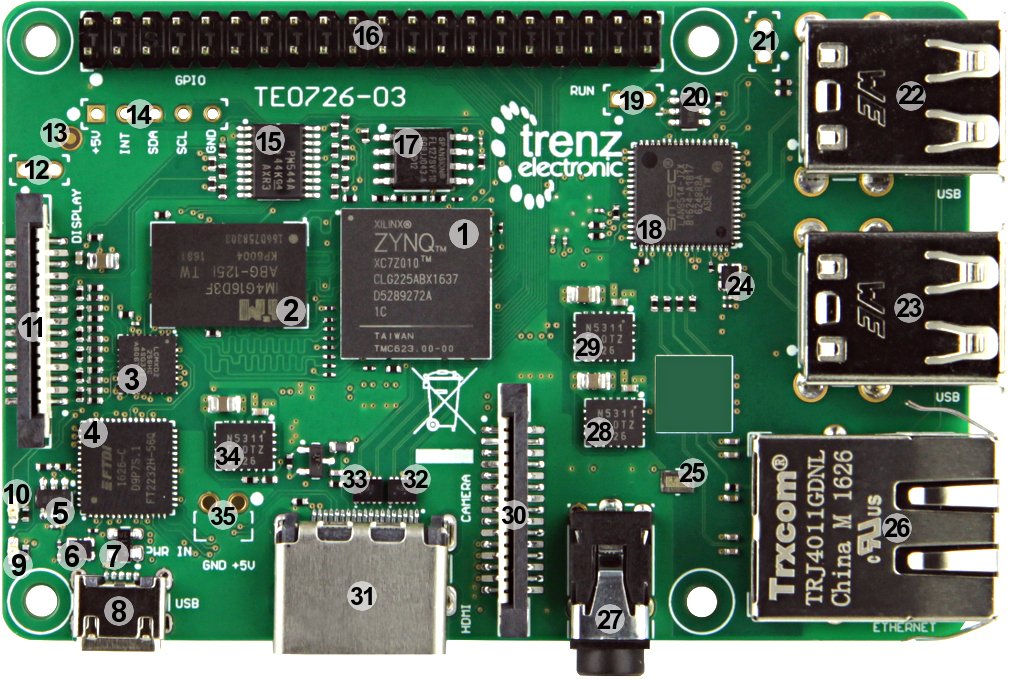
\includegraphics[width=0.5\textwidth]{zynqberry-top.png}
	\caption{Top view of the Znyqberry board, from \cite{zynq-main}.} \label{fig:znyqtop}
\end{figure}

The Zynqberry board, developed by the company Trenz Electronic GmbH, is a SoM (System on Module) based on the Xilinx All Programmable Zynq-700 SoC (XC7Z010) along with standar peripherials in an industrial-grade Raspberry Pi form factor. Some of the most relevant features are listed below \cite{zynq-main}:

\begin{itemize}
	\item Xilinx Zynq XC7Z010-1CLG225C
	\begin{itemize}
		\item 512 MByte DDR3L SDRAM
		\item 16 MByte Flash
	\end{itemize}
	\item Raspberry Pi Model 2 form factor
	\item LAN9514 USB hub with Ethernet
	\begin{itemize}
		\item 4 x USB with power switches
		\item 100 MBit Ethernet RJ45
	\end{itemize}
	\item Micro SD cad slot
	\item HAT header with 26 I/O's
	\item HDMI Type A
	\item DSI Connector (display)
	\item CSI-2 Connector (camera)
	\item Micro USB
	\begin{itemize}
		\item Power input
		\item USB UART
		\item JTAG ARM- and FPGA-Debug
	\end{itemize}
	\item 3.5 mm audio plug (PWM audio output only)
\end{itemize}

\begin{figure}
	\centering
	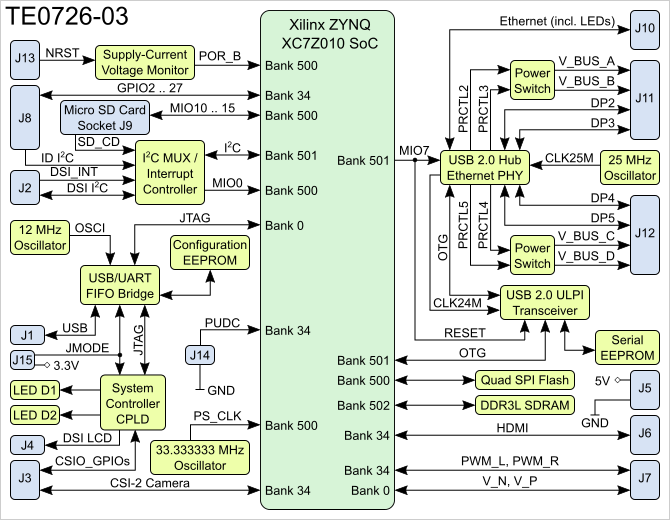
\includegraphics[width=0.7\textwidth]{zynq-block-diagram.png}
	\caption{Block diagram of the Zynqberry 726, from \cite{zynq-trm}.}	\label{fig:zynqblock}
\end{figure}

The physical device used in this project corresponds to the version 02 of the product, despite the fact that the manufacturer holds a newer 03 version. This needs to be considered during any reference consultation.

\section{Xilinx All Programmable Zynq-XC7Z010 SoC}

The Znyqberry TE-0726 02 board provides a SoC (System on Chip) device from the All Programmable Zynq-7000 family.

\subsection{Device Achitecture}

The Zynq-7000 SoC devices are part of the Xilinx All Programmable SoC architecture, integrating a dual-core ARM Cortex A9 processor (PS), and a 28 nm Xilinx programmable logic device (PL) into a single physical device. A general architectural diagram is shown in figure \ref{fig:zynq-arch-diag}

\begin{figure}
	\centering
	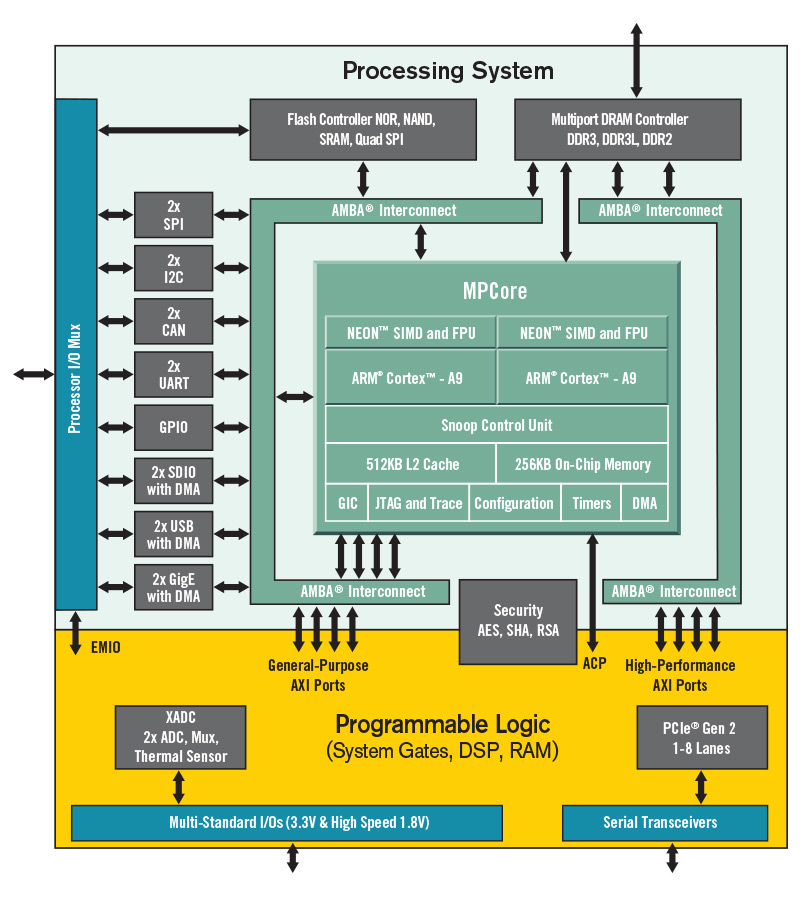
\includegraphics[width=0.7\textwidth]{zynq-arch-diag.png}
	\caption[Block diagram of the Zynq-7000 device family, from Xilinx Products Webpage.]{Architecture diagram of the Zynq-7000 device family, from Xilinx Products Webpage.\protect\footnotemark} \label{fig:zynq-arch-diag}
\end{figure}

\footnotetext{See \underline{https://www.xilinx.com/products/silicon-devices/soc/zynq-7000.html\#productAdvantages}}

\subsubsection{Processing System PS}

The Processing System (PS) is embedded into the FPGA device, providing and environment around it that makes possible more complex system configurations. The PS also includes on-chip memory and external memory interfaces. A more detailed characteristics description is available on \cite{DS190} and \cite{UG585}.

\begin{itemize}
	\item ARM Cortex-A9 Application Processor Unit
	\begin{itemize}
		\item 2.5 DMIPS/MHz per CPU
		\item CPU frequency up to 1GHz
		\item Single and double precision Vector Floating Point Unit (VFPU)
		\item Timer and interrupts
		\begin{itemize}
			\item Three watchdog timers
			\item One global timer
			\item Two triple-timer counters
		\end{itemize}
	\end{itemize}
	\item Cache
	\begin{itemize}
		\item 32kB Level 1 4-way set-associative instruction and data caches (cpu independent)
		\item 512 kB 8-way set associative Level 2 cache (CPU shared)
		\item Byte-parity support
	\end{itemize}
	\item On-chip memory
	\begin{itemize}
		\item On-chip boot ROM
		\item 256 kB on-chip RAM (OCM)
		\item Byte-parity support
	\end{itemize}
	\item External Memory Interfaces
	\begin{itemize}
		\item Multiprotocol dynamic memory controller
		\item 16-bit or 32-bit interfaces to DDR3, DDR3L, DDR2 or LPDDR2 memories
		\item ECC support in 16-bit Mode
		\item Static memory interfaces
		\begin{itemize}
			\item 8-bit SDRAM data bus qith up to 64 MB support
			\item Parallel NOR flash support
			\item ONFl1.0 NAND flash support (1-bit ECC)
			\item 1-bit SPI, 2-bit SPI, 4-bit SPI, or two quad-SPI (8-bit) serial NOR flash
		\end{itemize}
	\end{itemize}
	\item 8-Channel DMA controller
	\begin{itemize}
		\item Memory-to-memory, memory-to-peripherial, peripherial-to-memory and scatter-gather transaction support
	\end{itemize}
	\item I/O Peripherials and Interfaces
	\begin{itemize}
		\item Two 10/100/1000 tri-speed Ethernet MAC peripherials with IEEE Std 802.3 and IEEE Std 1588 revision 2.0 support
		\item Two USB 2.0 OTG peripherials, each supporting up to 12 Endpoints
		\begin{itemize}
			\item USB 2.0 compliant device IP core
			\item Supports on-the-go, high-speed, full-speed, and low-speed modes
			\item Intel EHCI compliant USB host
			\item 8-bit ULPI external PHY interfaces
		\end{itemize}
		\item Two full CAN 2.0B compliant CAN bus interfaces
		\begin{itemize}
			\item CAN 2.0-A and CAN 2.0-B and ISO 118981-1 Standar compliant
			\item External PHY interface
		\end{itemize}
		\item Two SD/SDIO 2.0/MMC3.31 compliant controllers
		\item Two full-duplex SPI ports with three peripherials chip selects
		\item Two high-speed UARTs (up to 1 Mb/s)
		\item Two mastar and slave I2C interfaces
		\item GPIO with four 32-bit banks, of which up to 54 bits can be used with the PS I/O (one bank of 32b and one bank of 22b) and up to 64 bits (up to two banks of 32b) connected to the Programmable Logic
		\item Up to 54 flexible multiplexed I/O (MIO) for peripherial pin assignments
	\end{itemize}
	\item Interconnect
	\begin{itemize}
		\item High-bandwidth connectivity within PS and PL
		\item ARM AMBA AXI based
		\item QoS support on critical masters for latency and bandwidth control
	\end{itemize}
\end{itemize}

\subsubsection{Programmable Logic PL}

\begin{itemize}
	\item Configurable Logic Blocks (CLB)
	\begin{itemize}
		\item Look-up tables (LUT)
		\item Flip-flops
		\item Cascadeable adders
	\end{itemize}
	\item 36 kb Block RAM
	\begin{itemize}
		\item True Dual-Port
		\item Up to 72 bits wide
		\item Configurable as dual 18 kb block RAM
	\end{itemize}
\end{itemize}

\section{Board Peripherials}

Based on the peripherials available on the Zynq XC7Z010, as well as the peripherials included in the board itself, a careful analysis needs to take place, given the fact that some of the peripherials in the SoC are not physicaly usable through the board, or that their functionality is already compromised for a specific purpose.

The case that is more relevant for this work, is the Ethernet controller available in the chip, that cannot be used due to the fact that the manufacturer uses a USB-to-Ethernet hub (See figure \ref{fig:zynqblock}, module right to the MIO7 connection). This means that for the development point of view, any Ethernet programming need to be done for the USB module, not the Ethernet one. Other limitations appear for any development, that need to be considered for future work.
